\section{Svartkroppsstrålning}
\label{sec:blackbody}

Alla objekt reflekterar, absorberar eller transmitterar ljus. De kroppar som varken 
reflekterar eller transmitterar något ljus utan absorberar $\unit[100]{\%}$ kallas konventionellt för svartkroppar. Detta är dock en teoretisk konstruktion då perfekta svartkroppar inte existerar men modellen kan ändå användas som en god modell i flera fysikaliska 
tillämpningar. Den energi som absorberats av kroppen strålas ut i form av svartkroppsstrålning vars 
frekvensspektrum bestäms av kroppens temperatur när kroppen är i termisk jämvikt med
 sin omgivning. Den totala utstrålade energin per tidsenhet fås ur Stefan-Boltzmanns lag
 
\begin{equation}
\label{eq:boltzmanslag}
\boxed{ \; \; \;
j^{\star} = \sigma T^{4}
\; \; \; }
\end{equation}

\noindent
där $\sigma$ är Stefan-Boltzmanns konstant som mäts i $\unit{W~m^{-2}~K^{-4}}$ och $T$ är kroppens temperatur vid termisk jämvikt.

\subsection{Härledning}
% av stefan-boltzmanns lag
% med hål i en låda
% kolla i termoboken
I en låda med fotoner kan den totala energin inne i lådan beskrivas som 
\begin{equation}
\label{eq:photonbox}
\frac{U}{V}=\frac{8\pi^5}{15}\frac{(kT)^4}{(hc)^3}
\end{equation}

där $U$ är  och $V$ är lådans volym. Ekvationen fås ur Plancks spektrum.\cite[ss.~301-302]{schroeder00} % Ev. förtydliga mer om vad som fås ur Plancks spektrum och vad U är.

Sedan görs ett litet hål i lådan, så att några av fotonerna kan slippa ut. Sannolikheten för att fotoner med kort respektive lång våglängd ska slippa ut är densamma som fördelningen mellan dem inne i lådan, eftersom de har samma hastighet.

Den totala mängden strålning som kommer ut kan då beräknas genom att tänka sig att 
de fotoner som når fram till hålet under en kort tidsperiod, $\mathrm{d}t$, alla befann sig
 på samma hemisfäriskt skal inne i lådan för en liten stund sedan, se figur \ref{fig:box}. Tjockleken på detta tänkta hemisfäriska skal är $c\mathrm{d}t$. Hemisfärens radie, $R$, beror givetvis på hur långt bakåt i tiden vi tittar.

\begin{figure}[hpbt]
\centering
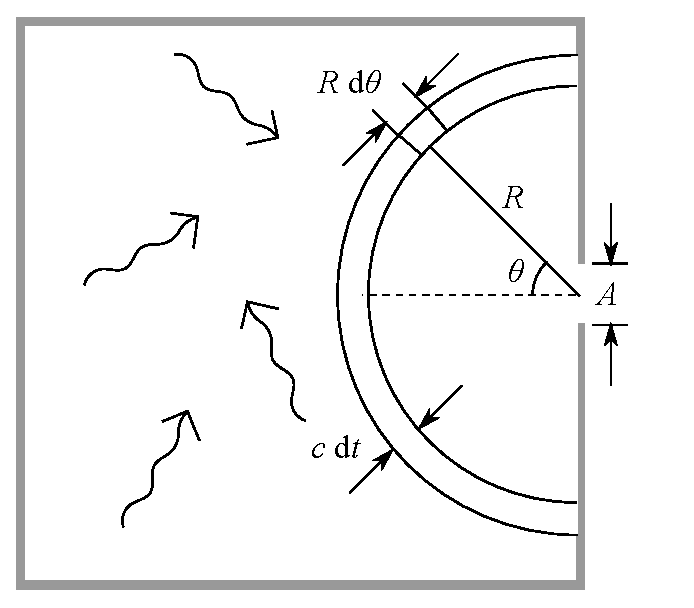
\includegraphics[height=5cm]{images/blackbody_box.eps}
\caption{\label{fig:box}{Fotonerna som lämnar lådan har en liten stund tidigare befunnit sig i samma hemisfär inne i lådan.}}
\end{figure}


Ett volymelement av det hemsfäriska skalet ges av
\begin{equation}
V=(R\mathrm{d}\theta) \times (R\sin\theta\mathrm{d}\phi) \times (c \mathrm{d}t).
\end{equation}

Energitätheten för fotonerna i volymelementet är således
\begin{equation}
E_\text{v.e.}=\frac{U}{V} c \mathrm{d}t R^2 \sin\theta \mathrm{d}\theta \mathrm{d}\phi.
\end{equation}

Men endast den andel av fotonerna som har rätt riktning kommer ut genom lådans öppning. Sannolikheten för att en foton har rätt riktning är
\begin{equation}
P(\text{rätt riktning})=\frac{A\cos\theta}{4\pi R^2}
\end{equation}

där A är hålets area. Den totala energin som strålar ut ur hålet från det lilla 
volymelementet är alltså 
\begin{equation}
\frac{A\cos\theta}{4\pi}\frac{U}{V} c\mathrm{d}t \sin\theta\mathrm{d}\theta \mathrm{d}\phi
\end{equation}

vilket ger en total energiutstrålning på
\begin{equation}
\frac{A}{4}\frac{U}{V}c \mathrm{d}t.
\end{equation}

Givetvis är utstrålningen beroende av både hålets area och tidsintervallet. Dividerar vi med dessa storheter får vi effekt per ytenhet, $j$,
\begin{equation}
j=\frac{c}{4}\frac{U}{V}. 
\end{equation}

Sätt in detta uttryck i ekvation~\eqref{eq:photonbox} så fås det vi känner som Stefan-Boltzmans lag,~\eqref{eq:boltzmanslag}
\begin{equation}
j=\frac{2\pi^5}{15}{(kT)^4}{h^3c^2}=\sigma T^4
\end{equation}

där $\sigma=\frac{2\pi^5k^4}{15h^3c^2}$ är Stefan-Boltzmans konstant.


\subsection{Strålning från omgivningen}
\label{sec:bb_sur}

\begin{figure}[hpbt]
\centering
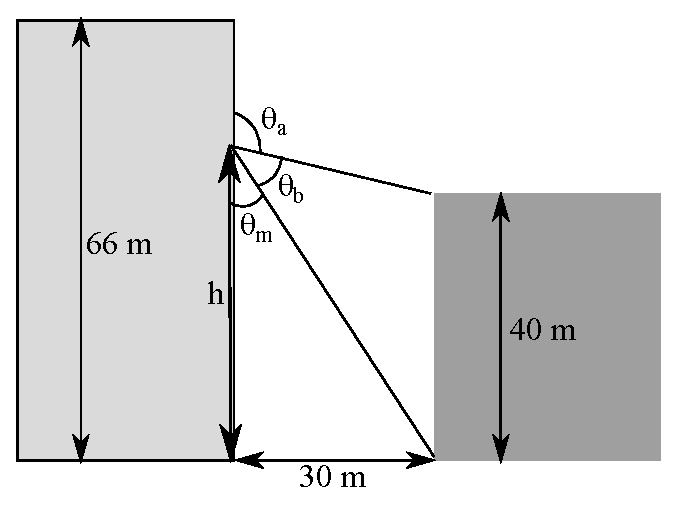
\includegraphics[height=4cm]{images/blackbody_surroundings.eps}
\caption{\label{fig:surroundings}{Den undersökta fastigheten på 
Wallerius\-gatan till vänster, och Johannebergs\-kyrkans församlings\-hem till höger. Den mot väggen instrålade svartkroppstrålningen kommer från olika källor. Här illustreras hur mycket av väggens omgivning som upptas mark, annan fastighet respektive atmosfären.}}
\end{figure}

För att uppskatta hur mycket svartkroppsstrålning som kommer mot väggen från olika 
delar av omgivningen sattes en enkel modell upp. Där antas att Johannebergskyrkans 
församlingshem ligger mitt emot vår undersökta fastighet på Walleriusgatan, att 
församlingshemmet ligger 30 meter bort och är 40 meter högt samt att det är det enda 
föremålet av betydande storlek i närheten, se figur~\ref{fig:surroundings}. För varje punkt
 på väggen beskrivs sedan hur stor andel av dess omgivning som upptas av marken, 
 församlingshemmet respektive himlen, eller atmosfären, med hjälp av ekvationerna

\begin{equation}
p_\text{gata}=\tan^{-1}(30/h)/180
\end{equation}

\begin{equation}
p_\text{byggnad}= \left\{
\begin{array}{rl}
\tan^{-1}(\frac{30}{h-40})/180 & \text{om } h > 40 \\
(\tan^{-1}(\frac{40-h}{30})+\tan^{-1}(\frac{h}{30}))/180^\circ & \text{om } h < 40 \\
\end{array} \right.
\end{equation}

\begin{equation}
p_\text{atmosfär}=1-p_\text{gata}-p_\text{byggnad}.
\end{equation}

Medelvärdet då $h$ går från 0 till 66 meter ger det genomsnittliga värdet för hur stor del av omgivningen som representeras av mark, annan fastighet och atmosfär för hela väggen. Detta ger resultatet att 26\% är gata, 36\% är 
 församlingshemmet och 38\% är atmosfären. Oftast antas allt som inte är atmosfären ha utomhustemperatur.

Ur \cite{bb_atmosphere} fås atmosfärens temperatur genom en modifierad variant av Stephan-Boltzmans lag och att strålningen från atmosfären en klar dag kan beskrivas som 
\begin{equation}
I_\text{atmosfär}=\sigma\cdot T_\text{ute}^4(1-c \cdot e^{-d(273-T_\text{ute})^2})
\end{equation}
där $c=0,261$ och $d=7,77\cdot10^{-4}$ kommer ur statistiska data. En helt molnig dag är atmosfärens temperatur samma som utomhustemperaturen, $T_\text{ute}$, det vill säga $c=0$. Denna ekvation har fåtts ut statistiska data och visar sig stämma bra för hela världen\cite{bb_atmosphere}.